\documentclass[10pt,twocolumn,letterpaper]{article}

\usepackage{iccv}
\usepackage{times}
\usepackage{epsfig}
\usepackage{graphicx}
\usepackage{amsmath}
\usepackage{amssymb}
\usepackage{algorithm}
\usepackage{algorithmic}
\usepackage{bbm}
\usepackage{amsfonts}
\usepackage{mathrsfs}
\usepackage{multirow}
\usepackage{graphicx}
\usepackage{booktabs}

% Include other packages here, before hyperref.

% If you comment hyperref and then uncomment it, you should delete
% egpaper.aux before re-running latex.  (Or just hit 'q' on the first latex
% run, let it finish, and you should be clear).

\usepackage[pagebackref=true,breaklinks=true,letterpaper=true,colorlinks,bookmarks=false]{hyperref}


\iccvfinalcopy % *** Uncomment this line for the final submission

\def\iccvPaperID{406} % *** Enter the CVPR Paper ID here
\def\httilde{\mbox{\tt\raisebox{-.5ex}{\symbol{126}}}}

% Pages are numbered in submission mode, and unnumbered in camera-ready


\begin{document}

%%%%%%%%% TITLE
\title{\LARGE{Novel View Synthesis: A Review and Taxonomy Focused on Neural Radiance Fields (NeRF)}}  \vspace{-10pt}

\author{22281188 Jiawei Jiang{$^{1}$}\\\vspace{-10pt}{\small~}\\
{$^{1}$}Beijing Jiaotong University;\\
{\small{{$^{*}$}Student Email: \tt{22281188@bjtu.edu.cn}}}
}
% For a paper whose authors are all at the same institution,
% omit the following lines up until the closing ``}''.
% Additional authors and addresses can be added with ``\and'',
% just like the second author.
% To save space, use either the email address or home page, not both



\maketitle
\thispagestyle{empty}







\begin{abstract}
Novel View Synthesis (NVS), the generation of images from new viewpoints based on existing input views, is a cornerstone problem in computer vision and graphics with wide-ranging applications. This paper presents a comprehensive survey charting the evolution of NVS methodologies. This paper traces the historical progression through four distinct eras: early techniques rooted in geometric principles and Multi-View Stereo (MVS) (c. 2000-2010); the advent of regression-based deep learning approaches (c. 2010-2017); the rise of powerful generative models like GANs and Transformers (c. 2018-2022); and the current wave of diffusion model-based synthesis (c. 2021-present). Subsequently, this paper provide an in-depth analysis of Neural Radiance Fields (NeRF), a paradigm-shifting technique that has recently dominated the field. This paper discuss the specific application requirements driving NeRF research, delineate key challenges including model capacity allocation, noise handling, few-shot learning, and computational efficiency, and summarize corresponding solution strategies. Furthermore, I offer a structured taxonomy of contemporary NeRF-related works, categorizing them based on their focus on large-scale scenes, dynamic elements and complex lighting, few-shot reconstruction, and computational acceleration. This survey serves as a valuable resource for understanding the NVS landscape and navigating the rapidly expanding NeRF literature.\end{abstract}
% Keywords: Novel View Synthesis, Neural Radiance Fields, Generative Models, Diffusion Models, Computer Vision

% 确保在导言区加载了 graphicx 宏包
% \usepackage{graphicx}

\begin{figure*}[t] % 使用 figure* 实现全宽,[t] 建议放在顶部
    \centering % 图像居中
    \includegraphics[
        width=\textwidth,        % 设置显示宽度为文本宽度
        trim={0cm 3cm 2cm 1.2cm}, % 【关键】裁切量:左 下 右 上 - 请根据你的图片调整这些数值!
        clip                     % 应用裁切
    ]{./fig/3.pdf}             % 【检查】确保图片路径和文件名正确!
    \caption{Timeline illustrating the evolution of Novel View Synthesis (NVS). Key phases include Geometric Methods, Learned Regression, Generative Models, the NeRF Revolution, and Diffusion Models \& Hybrids.} % 标题
    % --- 修改了标签以确保唯一性 ---
    \label{fig:nvs_timeline_figure} % 使用唯一的标签
    % --- 标签修改结束 ---
\end{figure*}

\section{Introduction}

Novel View Synthesis (NVS), the task of generating photorealistic images of a scene from arbitrary viewpoints given a set of input views, stands as a fundamental challenge in computer vision and computer graphics. Its applications are widespread, ranging from immersive virtual and augmented reality (VR/AR) experiences and robotics to visual effects and digital content creation. The core challenge lies in inferring the underlying 3D scene structure and appearance from limited, often sparsely sampled, visual data to render plausible novel perspectives.

Early approaches to NVS were predominantly geometry-based, relying heavily on classical Structure-from-Motion (SfM) and Multi-View Stereo (MVS) techniques to explicitly reconstruct 3D scene geometry (e.g., point clouds, meshes, or depth maps) \cite{snavely2006photo, goesele2007multi}. While foundational, these methods often struggle to produce highly photorealistic renderings, particularly in regions with complex non-Lambertian surfaces, intricate details, or significant occlusions. Furthermore, the quality of the synthesized views is critically dependent on the accuracy of the intermediate geometric reconstruction, which can be fragile.
% Note: Added a generic citation placeholder for the summary point if needed

The advent of deep learning ushered in a new era for NVS. Regression-based methods emerged, leveraging convolutional neural networks (CNNs) to directly predict novel view images \cite{flynn2016deepstereo}. Many subsequent works integrated learned components with 3D representations and differentiable rendering pipelines \cite{kato2018neural}. While initially often scene-specific, significant progress has been made towards few-shot NVS, enabling generalization across scenes from only one or a few input images, sometimes employing meta-learning or test-time optimization strategies \cite{yu2021pixelnerf}. % Note: Added a generic citation placeholder for the summary point if needed

Concurrently, generative models gained traction, particularly for challenging scenarios involving large viewpoint extrapolation where geometric priors might be weak or absent \cite{wiles2020pixelsynth, rombach2021geometry}. These models excel at synthesizing plausible scene content by learning powerful priors from data, capable of filling in significant missing information \cite{niemeyer2021giraffe, ren2022look}. 3D Generative Adversarial Networks (GANs) also demonstrated capability in generating 3D objects, although often limited to object-centric setups and canonical poses \cite{wu2016learning}. However, maintaining long-range geometric and temporal consistency remained a challenge for purely generative approaches without strong 3D guidance.

A pivotal moment arrived with the introduction of Neural Radiance Fields (NeRF) \cite{mildenhall2020nerf}. By representing a scene as a continuous volumetric function optimized via neural networks and rendered using differentiable volume rendering, NeRF achieved unprecedented photorealism and view consistency. This breakthrough spurred a massive wave of research, establishing NeRF as a cornerstone of modern NVS.

Most recently, diffusion models \cite{dhariwal2021diffusion}, initially demonstrating state-of-the-art performance in 2D image synthesis, have been successfully adapted for NVS and 3D-aware generation \cite{poole2022dreamfusion, watson2022novel}. These methods often combine the generative power of diffusion with geometric priors or integrate with NeRF-like representations, aiming to achieve both realism and multi-view consistency \cite{kulhanek2023consistent}. % Note: Added a generic citation placeholder for the summary point if needed

This paper provides a comprehensive survey of the evolution of Novel View Synthesis techniques. It traces the trajectory from early geometric foundations through the rise of deep learning-based regression and generative models, culminating in the current landscape dominated by Neural Radiance Fields and diffusion models. The primary focus of this paper is an in-depth analysis of NeRF-based approaches. This paper systematically discuss the application demands driving NeRF development, identify the core challenges encountered (e.g., foreground/background ambiguity, handling dynamic elements, optimizing from limited samples, computational cost), review proposed solution strategies (e.g., decomposition, appearance modeling, priors, architectural optimizations), and provide a structured taxonomy of the burgeoning NeRF literature. This includes works focusing on large-scale unbounded scenes \cite{barron2022mipnerf360, turki2022mega}, handling dynamic scenes and complex illumination \cite{martinbrualla2021nerfw, tancik2022blocknerf}, reconstructing from few input views \cite{chen2021mvsnerf, jain2021dietnerf, yang2023freenerf}, and accelerating training and inference \cite{yu2021plenoctrees, fridovichkeil2022plenoxels, mueller2022instant}. By contextualizing NeRF within the broader history of NVS and organizing its variants, this survey aims to offer a valuable resource for researchers and practitioners navigating this rapidly evolving field.

\section{Related Works}
\noindent\textbf{Pose or viewpoint estimation} has a long history in computer vision \cite{murphy2009head}. It arises in different applications, such as head \cite{murphy2009head}, pedestrian body \cite{raza2018appearance}, vehicle \cite{yang2018hierarchical} and object class \cite{su2015render} orientation/pose estimation. Although these systems are mostly developed independently, they are essentially the same problem in our framework.

The current related literature using deep networks can be divided into two categories. Methods in the first group, such as \cite{rad2017bb8,grabner20183d,zhou2018starmap}, predict keypoints in images and then recover the pose using pre-defined 3D object models. The keypoints can be either semantic \cite{pavlakos20176,wu2016single,massa2016crafting} or the eight corners of a 3D bounding box encapsulating the object \cite{rad2017bb8,grabner20183d}. 

The second category of methods, which are more close to our approach, estimate angular values directly from the image \cite{elhoseiny2016comparative,wang2016viewpoint}. Instead of the typical Euler angle representation for rotations \cite{elhoseiny2016comparative}, biternion representation is chosen in \cite{beyer2015biternion,prokudin2018deep} and inherits the periodicity in its $sin$ and $cos$ operations. However, their setting is compatible with only the regression. Several studies have evaluated the performance of classification and regression-based loss functions and conclude that the classification methods usually outperform the regression ones in pose estimation \cite{massa2016crafting,mahendran2018mixed}. 

These limitations were also found in the recent approaches which combine classification with regression or even triplet loss \cite{mahendran2018mixed,yang2018hierarchical}.



\noindent\textbf{Wasserstein distance} is a measure defined between probability distributions on a given metric space \cite{kolouri2016sliced}. Recently, it attracted much attention in generative models $etc$ \cite{arjovsky2017wasserstein}. \cite{frogner2015learning} introduces it for multi-class multi-label task with a linear model. Because of the significant amount of computing needed to solve the exact distance for general cases, these methods choose the approximate solution, whose complexity is still in $\mathcal{O}(N^2)$ \cite{cuturi2013sinkhorn}. The fast computing of discrete Wasserstein distance is also closely related to SIFT \cite{cha2002measuring} descriptor, hue in HSV or LCH space \cite{cha2002fast} and sequence data \cite{su2017order}. Inspired by the above works, we further adapted this idea to the pose estimation, and encode the geometry of label space by means of the ground matrix. We show that the fast algorithms exist in our pose label structure using the one-hot or conservative target label and the ground metric is not limited to the arc length. 







\noindent\textbf{Robust training with noise data} has long been studied for general classification problems \cite{huber2011robust}. Smoothing the one-hot label \cite{szegedy2016rethinking} with a uniform distribution or regularizing the entropy of softmax output \cite{pereyra2017regularizing} are two popular solutions. Some works of regression-based localization model the uncertainty of point position in a plane with a 2D Gaussian distribution \cite{szeto2017click}. \cite{zou2019confidence} propose to regularize self-training with confidence. However, there are few studies for the discrete periodic label. Besides sampling on Gaussian, the Poisson and the Binomial distribution are further discussed to form a unimodal-uniform distribution.



\noindent\textbf{Uncertainty quantification of pose estimation} aims to quantify the reliability of a result $e.g.,$ a confidence distribution of each class rather than a certain angle value for pose data \cite{prokudin2018deep}. A well-calibrated uncertainty is especially important for large systems to assess the consequence of a decision \cite{che2019deep,han2019unsupervised}. \cite{prokudin2018deep} proposes to output numerous sets of the mean and variation of Gaussian/Von-Mises distribution following \cite{beyer2015biternion}. It is unnecessarily complicated and is a somewhat ill-matched formulation as it assumes the pose label is continuous, while it is discrete. We argue that the $softmax$ is a natural function to capture discrete uncertainty, and is compatible with Wasserstein training.



\section{Methodology}

We consider learning a pose estimator ${h}_\theta$, parameterized by $\theta$, with $N$-dimensional softmax output unit. It maps a image {\rm\textbf{x}} to a vector ${\rm\textbf{s}}\in\mathbb{R}^N$. We perform learning over a hypothesis space $\mathcal{H}$ of ${h}_\theta$. Given input {\rm\textbf{x}} and its target ground truth one-hot label ${\rm\textbf{t}}$, typically, learning is performed via empirical risk minimization to solve $\mathop{}_{{h}_\theta\in\mathcal{H}}^{\rm min}\mathcal{L}({h}_\theta({\rm\textbf{x}}),{\rm\textbf{t}})$, with a loss $\mathcal{L}(\cdot,\cdot)$ acting as a surrogate of performance measure.

Unfortunately, cross-entropy, information divergence, Hellinger distance and $\mathcal{X}^2$ distance-based loss treat the output dimensions independently \cite{frogner2015learning}, ignoring the similarity structure on pose label space.  

Let ${\rm\textbf{s}}=\left\{s_i\right\}_{i=0}^{N-1}$ be the output of ${h}_\theta({\rm\textbf{x}})$, $i.e.,$ softmax prediction with $N$ classes (angles), and define ${\rm\textbf{t}}=\left\{t_j\right\}_{j=0}^{N-1}$ as the target label distribution, where $i,j\in\left\{0,\cdots,{\small N-1}\right\}$ be the index of dimension (class). Assume class label possesses a ground metric ${\rm\textbf{D}}_{i,j}$, which measures the semantic similarity between $i$-th and $j$-th dimensions of the output. There are $N^2$ possible ${\rm\textbf{D}}_{i,j}$ in a $N$ class dataset and form a ground distance matrix $\textbf{D}\in\mathbb{R}^{N\times N}$. When ${\rm\textbf{s}}$ and ${\rm\textbf{t}}$ are both histograms, the discrete measure of exact Wasserstein loss is defined as \begin{equation}
\mathcal{L}_{\textbf{D}_{i,j}}({\rm{\textbf{s},\textbf{t}}})=\mathop{}_{\textbf{W}}^{{\rm inf}}\sum_{j=0}^{N-1}\sum_{i=0}^{N-1}\textbf{D}_{i,j}\textbf{W}_{i,j} \label{con:df}
\end{equation} where \textbf{W} is the transportation matrix with \textbf{W}$_{i,j}$ indicating the mass moved from the $i^{th}$ point in source distribution to the $j^{th}$ target position. A valid transportation matrix \textbf{W} satisfies: $\textbf{W}_{i,j}\geq 0$; $\sum_{j=0}^{N-1}\textbf{W}_{i,j}\leq s_i$; $\sum_{i=0}^{N-1}\textbf{W}_{i,j}\leq t_j$; $\sum_{j=0}^{N-1}\sum_{i=0}^{N-1}\textbf{W}_{i,j}={\rm min}(\sum_{i=0}^{N-1}s_i,\sum_{j=0}^{N-1}t_j)$.



The ground distance matrix ${\rm\textbf{D}}$ in Wasserstein distance is usually unknown, but it has clear meanings in our application. Its $i,j$-th entry ${\rm\textbf{D}}_{i,j}$ could be the geometrical distance between the $i$-th and $j$-th points in a circle. A possible choice is using the arc length ${d_{i,j}}$ of a circle ($i.e., \ell_1$ distance between the $i$-th and $j$-th points in a circle) as the ground metric $\textbf{D}_{i,j}={d_{i,j}}$.

\begin{equation}
d_{i,j}={\rm min}\left\{|i-j|,N-|i-j|\right\} \label{con:d}
\end{equation}  


The Wasserstein distance is identical to the Earth mover's distance when the two distributions have the same total masses ($i.e., \sum_{i=0}^{N-1}s_i=\sum_{j=0}^{N-1}t_j$) and using the symmetric distance $d_{i,j}$ as ${\rm\textbf{D}}_{i,j}$.



This setting is satisfactory for comparing the similarity of SIFT or hue \cite{rubner2000earth}, which do not use a neural network optimization. The previous efficient algorithm usually holds only for $\textbf{D}_{i,j}={d_{i,j}}$. We propose to extend the ground metric in ${\rm\textbf{D}}_{i,j}$ as $f(d_{i,j})$, where $f$ is a positive increasing function $w.r.t.$ $d_{i,j}$. 






 

% \subsection{Wasserstein training with one-hot target}



% The one-hot encoding is a typical setting for multi-class one-label dataset. The distribution of a target label probability is ${\rm\textbf{t}}=\delta_{j,j^*}$, where $j^*$ is the ground truth class, $\delta_{j,j^*}$ is a Dirac delta, which equals to 1 for $j=j^*$\footnote{\noindent We use $i,j$ interlaced for ${\rm \textbf{s}}$ and ${\rm \textbf{t}}$, since they index the same group of positions in a circle.}, and $0$ otherwise. 

% \begin{figure}[t]
% \centering
% \begin{tabular}{cc}
% 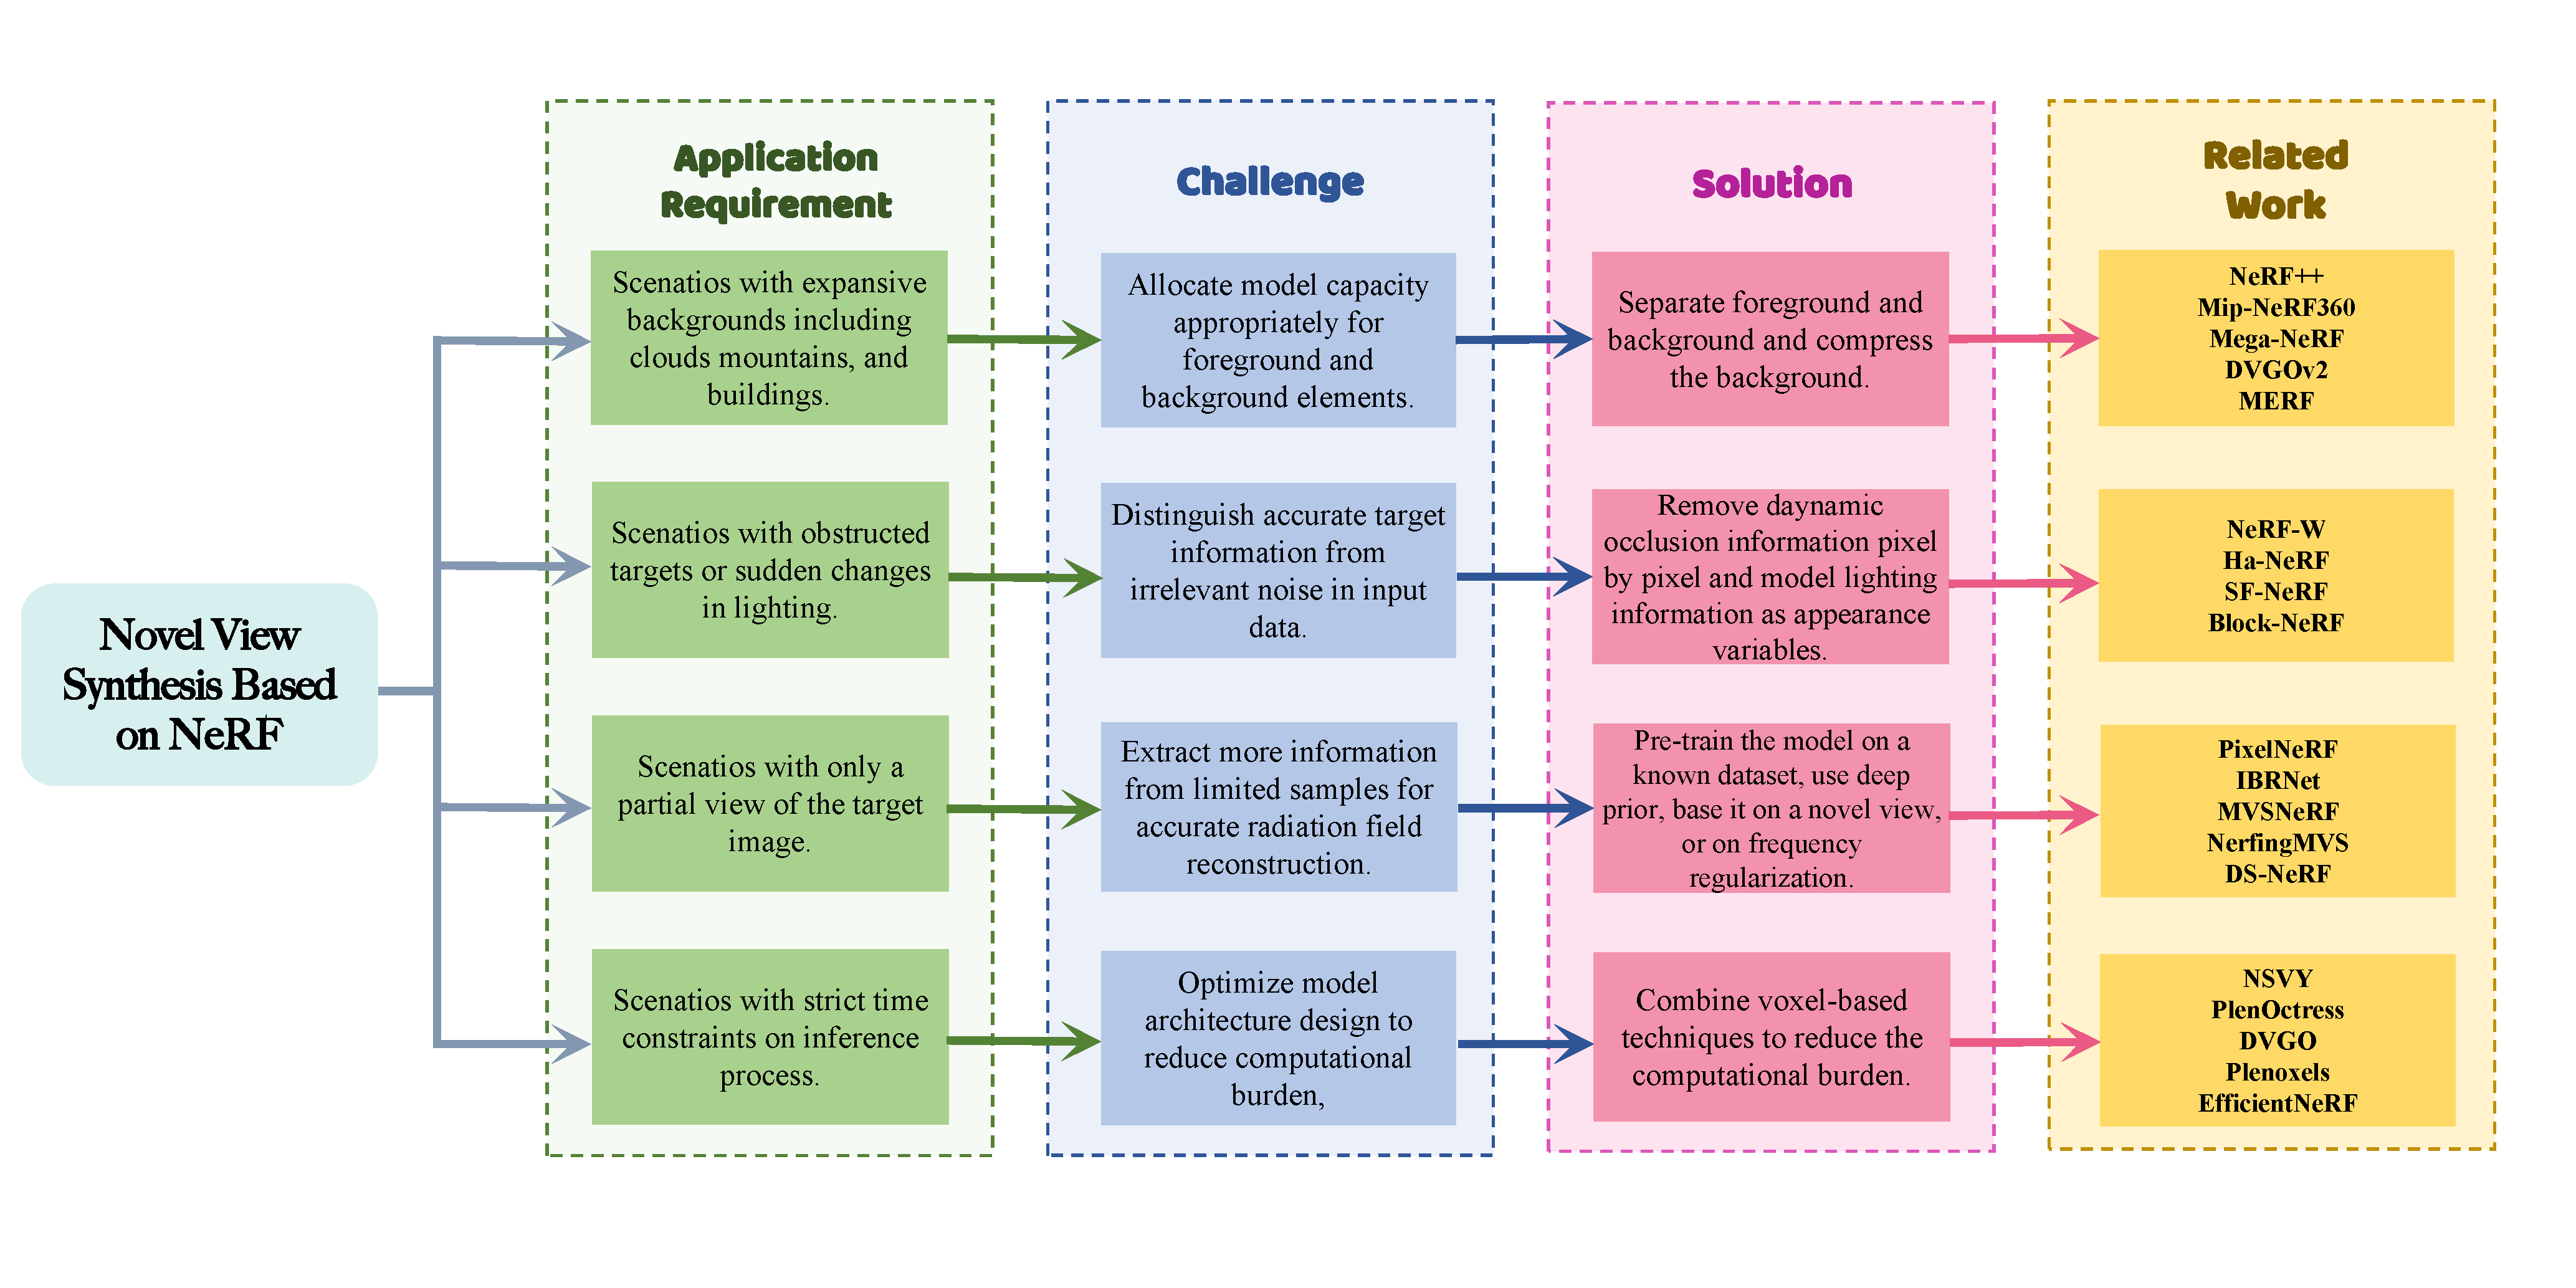
\includegraphics[height=6.8cm]{fig/NeRF.pdf}&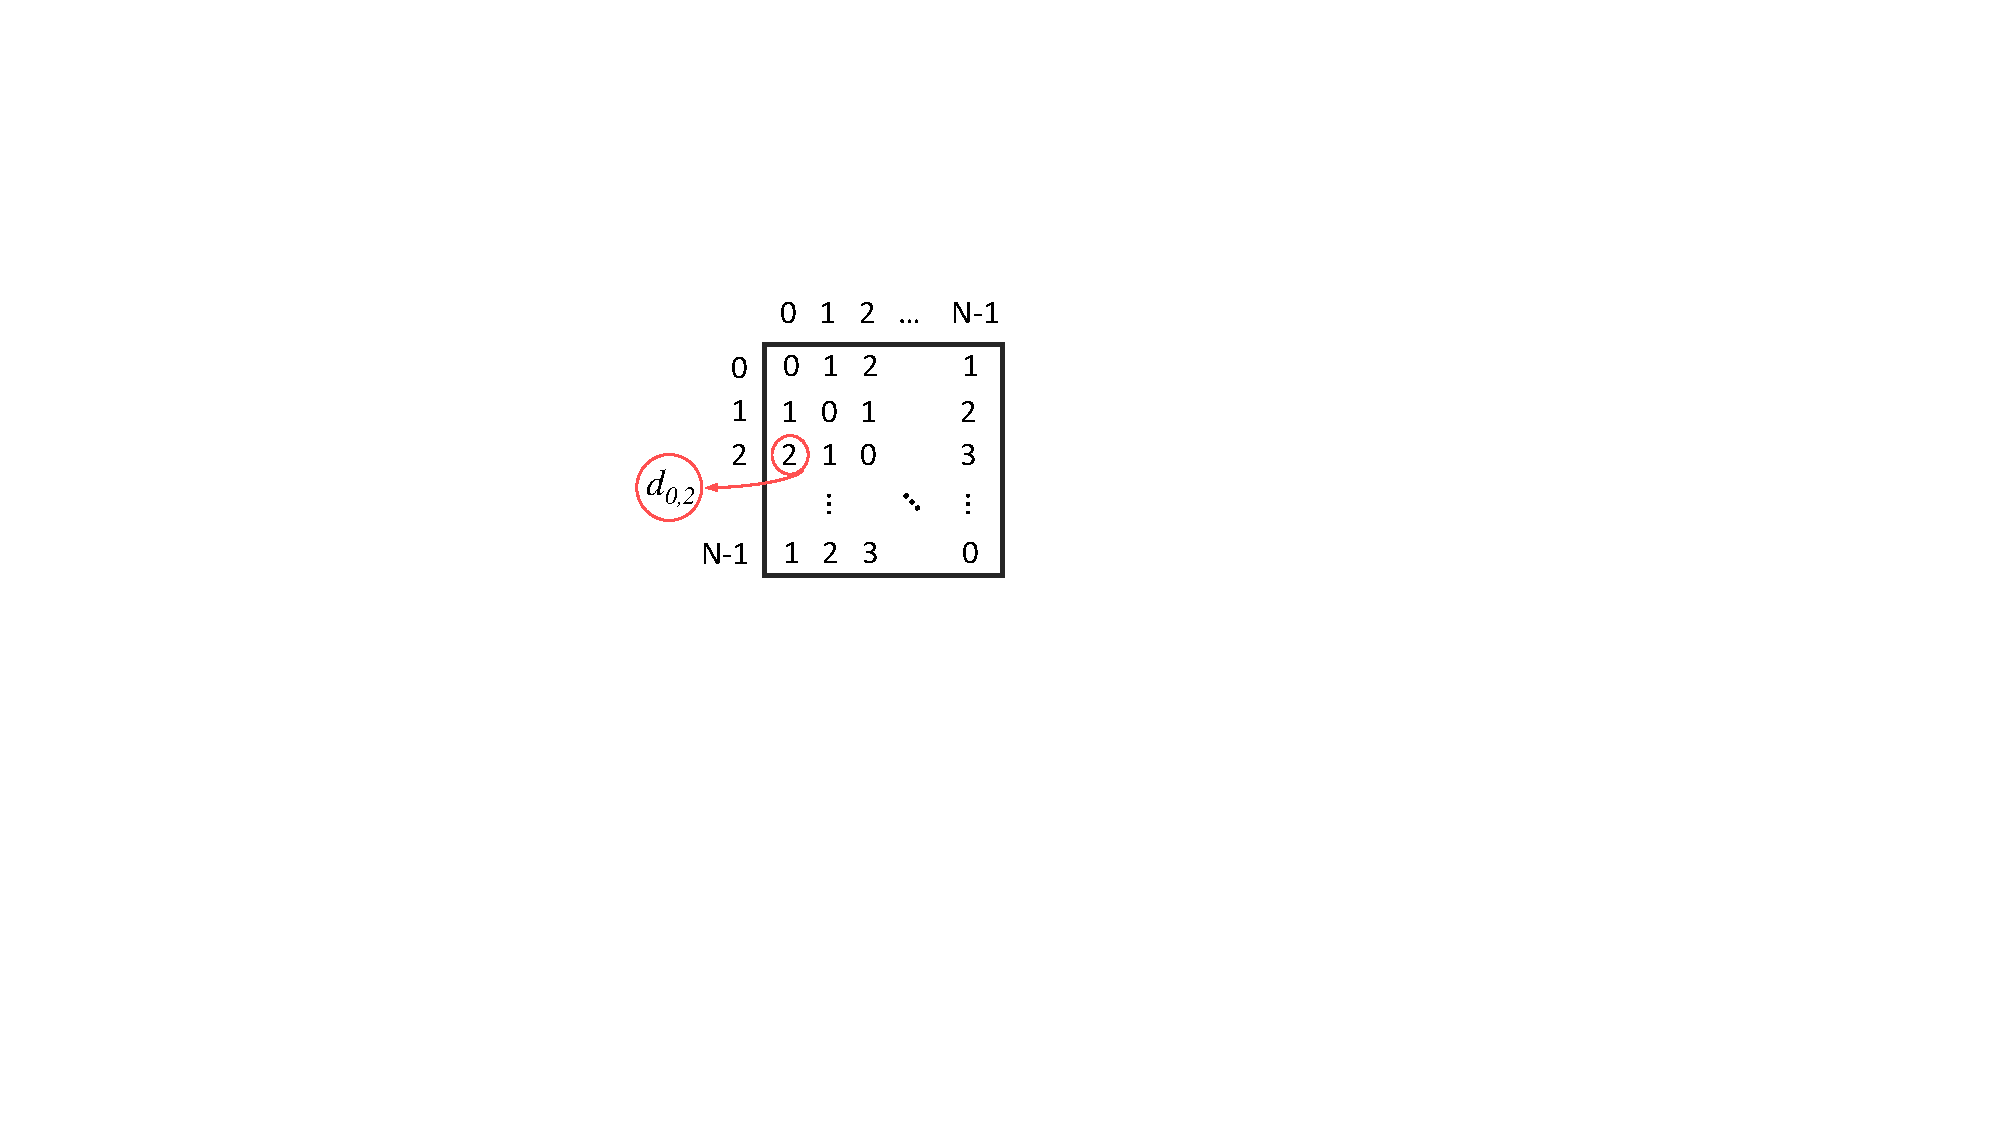
\includegraphics[height=2.8cm]{fig//fig2_2.pdf}
% \end{tabular}
% \caption{Left: The only possible transport plan in one-hot target case. Right: the ground matrix using arc length as ground metric.}
% \label{fig:2}
% \end{figure} 

% \noindent\textbf{Theorem 1.} \textit{Assume that} $\sum_{j=0}^{N-1}t_j=\sum_{i=0}^{N-1}s_i$, \textit{and} ${\rm{\textbf{t}}}$ \textit{is a one-hot distribution with} $t_{j^*}=1 ($or $\sum_{i=0}^{N-1}s_i)$\footnote{We note that softmax cannot strictly guarantee the sum of its outputs to be 1 considering the rounding operation. However, the difference of setting $t_{j^*}$ to $1$ or $\sum_{i=0}^{N-1}s_i)$ is not significant in our experiments using the typical format of softmax output which is accurate to 8 decimal places.}, \textit{there is only one feasible optimal transport plan.} 



% According to the criteria of ${\rm\textbf{W}}$, all masses have to be transferred to the cluster of the ground truth label $j^*$, as illustrated in Fig. \ref{fig:2}. Then, the Wasserstein distance between softmax prediction {\rm{\textbf{s}}} and one-hot target {\rm{\textbf{t}}} degenerates to\begin{equation}
% \mathcal{L}_{{\rm\textbf{D}}_{i,j}^{f}}({\rm{\textbf{s},\textbf{t}}})=\sum_{i=0}^{N-1} s_i f(d_{i,j^*}) \label{con:df}
% \end{equation} where ${\rm\textbf{D}}_{i,j}^f=f(d_{i,j})$. Practically, $f$ can be an increasing function proper, $e.g., p^{th}$ power of $d_{i,j}$ and Huber function. The exact solution of Eq. \eqref{con:df} can be computed with a complexity of $\mathcal{O}(N)$. The ground metric term $f(d_{i,j^*})$ works as the weights $w.r.t.$ $s_i$, which takes all classes into account following a soft attention scheme \cite{liu2018dependency,liu2019dependency,liu2019permutation}. It explicitly encourages the probabilities distributing on the neighboring classes of $j^*$. Since each $s_i$ is a function of the network parameters, differentiating $\mathcal{L}_{{\rm\textbf{D}}_{i,j}^{f}} w.r.t.$ network parameters yields $\sum_{i=0}^{N-1}s_i'f(d_{i,j^*})$.    



% In contrast, the cross-entropy loss in one-hot setting can be formulated as $-1{\rm log}s_{j^*}$, which only considers a single class prediction like the hard attention scheme \cite{liu2018dependency,liu2019dependency,liu2019permutation}, that usually loses too much information. Similarly, the regression loss using softmax prediction could be $f(d_{i^*,j^*})$, where $i^*$ is the class with maximum prediction probability.


% In addition to the predefined ground metric, we also propose to learn ${\rm\textbf{D}}$ adaptively along with our training following an alternative optimization scheme \cite{liu2018joint}.

% \noindent\textbf{Step 1:} Fixing ground matrix ${\rm\textbf{D}}$ to compute $\mathcal{L}_{{\rm\textbf{D}}_{i,j}}({\rm{\textbf{s},\textbf{t}}})$ and updating the network parameters.

% \noindent\textbf{Step 2:} Fixing network parameters and postprocessing ${\rm\textbf{D}}$ using the feature-level $\ell_1$ distances between different poses.

% We use the normalized second-to-last layer neural response in this round as feature vector, since there is no subsequent non-linearities. Therefore, it is meaningful to average the feature vectors in each pose class to compute their centroid and reconstruct ${{\rm\textbf{D}}_{i,j}}$ using the $\ell_1$ distances between these centroids $\overline{d}_{i,j}$. To avoid the model collapse, we construct the ${{\rm\textbf{D}}_{i,j}=\frac{1}{1+\alpha}\left\{f(\overline{d}_{i,j})+\alpha f(d_{i,j})\right\}}$ in each round, and decrease $\alpha$ from 10 to 0 gradually in the training.   
 

 









\subsection{Wrapped unimodal-uniform smoothing}



The outlier noise exists in most of data-driven tasks, and can be modeled by a uniform distribution \cite{szegedy2016rethinking}. However, pose labels are more likely to be mislabeled as a close class of the true class. It is more reasonable to construct a unimodal distribution to depict the inlier noise in pose estimation, which has a peak at class $j^*$ while decreasing its value for farther classes. We can sample on a continuous unimodal distribution ($e.g.,$ Gaussian distribution) and followed by normalization, or choose a discrete unimodal distribution ($e.g.,$ Poisson/Binomial distribution). 


\noindent\textbf{Gaussian/Von-Mises Distribution} has the probability density function (PDF) $f(x)=\frac{{\rm{exp}}\left\{-(x-\mu)^2/2\sigma^2\right\}}{\sqrt{2\pi\sigma^2}}$ for $x\in [0,\small K]$, where $\mu=K/2$ is the mean, and $\sigma^{2}$ is the variance. Similarly, the Von-Mises distribution is a close approximation to the circular analogue of the normal distribution ($i.e., \small K=N-1$). We note that the geometric loss \cite{su2015render} is a special case, when we set $\xi=1,\eta=0$, $\small{K=N-1}$, remove the normalization and adopt CE loss. Since we are interested in modeling a discrete distribution for target labels, we simply apply a softmax operation over their PDF. Note that the output values are mapped to be defined on the circle.

 

\noindent\textbf{Poisson Distribution} is used to model the probability of the number of events, $k$ occurring in a particular interval of time. Its probability mass function (PMF) is:\vspace{-5pt}\begin{equation}
p_k=\frac{\lambda^k{\rm{exp}}(-\lambda)}{k!},~~~k= 0, 1, 2, ...,       
\end{equation}\vspace{-2pt}where $\lambda\in \mathbb{R}^+$ is the average frequency of these events. We can sample $K+1$ probabilities ($i.e., 0\leq k\leq K$) on this PMF and followed by normalization for discrete unimodal probability distributions. Since its mean and variation are the same ($i.e., \lambda$), it maybe inflexible to adjust its shape.     


\noindent\textbf{Binomial Distribution} is commonly adopted to model the probability of a given number of successes out of a given number of trails $k$ and the success probability $p$.\vspace{-5pt}\begin{equation}
p_k={n\choose k}p^k(1-p)^{n-k},~~~n\in\mathbb{N},~~k=0,1,2, ...,n
\end{equation}\vspace{-2pt}We set $n=K$ to construct a distribution with $K+1$ bins without softmax normalization. Its warp processing with $K=20$ is illustrated in Fig. \ref{fig:3}.


\begin{figure}[t]
\centering
\includegraphics[width=8.2cm]{fig//fig3.pdf}\\
\caption{Left: the wrapping operation with a Binomial distribution ($\small K+1$ is the number of involved classes of unimodal distribution). Right: the distribution of conservative target label.}\label{fig:3}
\end{figure}

The conservative target distribution ${\rm{{\overline{\textbf{t}}}}}$ is constructed by replacing $t_{j}$ in ${\rm\textbf{t}}$ with $(1-\xi-\eta)t_{j}+\xi p_j +\eta \frac{1}{N}$, which can be regarded as the weighted sum of the original label distribution ${\rm\textbf{t}}$ and a unimodal-uniform mixture distribution. When we only consider the uniform distribution and utilize the CE loss, it is equivalent to label smoothing \cite{szegedy2016rethinking}, a typical mechanism for outlier noisy label training, which encourages the model to accommodate less-confident labels. 


By enforcing {\rm\textbf{s}} to form a unimodal-uniform mixture distribution, we also implicitly encourage the probabilities to distribute on the neighbor classes of $j^*$.


 















\subsection{Wasserstein training with conservative target}

With the conservative target label, the fast computation of Wasserstein distance in Eq. \eqref{con:df} does not apply. A straightforward solution is to regard it as a general case and solve its closed-form result with a complexity higher than $\mathcal{O}(N^3)$ or get an approximate result with a complexity in $\mathcal{O}(N^2)$. The main results of this section are a series of analytic formulation when the ground metric is a nonnegative increasing linear/convex/concave function $w.r.t.$ arc length with a reasonable complexity.\\





\noindent\textbf{3.3.1 Arc length $d_{i,j}$ as the ground metric.}


When we use $d_{i,j}$ as ground metric directly, the Wasserstein loss $\mathcal{L}_{d_{i,j}}(\rm{\textbf{s},\overline{\textbf{t}}})$ can be written as \begin{equation}
\mathcal{L}_{d_{i,j}}{(\rm{{\textbf{s},\overline{\textbf{t}}}})=\mathop{}_{\alpha\in\mathbb{R}}^{inf}}\sum_{j=0}^{N-1}|{\sum_{i=0}^{j}(s_i-\overline{{t}}_i)}-\alpha|\label{con:medi}
\end{equation}

To the best of our knowledge, Eq. \eqref{con:medi} was first developed in \cite{werman1986bipartite}, in which it is proved for sets of points with unitary masses on the circle. A similar conclusion for the Kantorovich-Rubinstein problem was derived in \cite{cabrelli1995kantorovich,cabrelli1998linear}, which is known to be identical to the Wasserstein distance problem when ${{\rm\textbf{D}}_{i,j}}$ is a distance. We note that this is true for $\mathcal{L}_{d_{i,j}}$ (but false for $\mathcal{L}_{{\rm\textbf{D}}^{\rho}}{(\rm{{\textbf{s},\overline{\textbf{t}}}})}$ with $\rho>1$). The optimal $\alpha$ should be the median of the set values $\left\{\sum_{i=0}^{j}(s_i-\overline{{t}}_i), 0\leq j\leq {\scriptsize{N}}-1\right\}$ \cite{pele2008linear}. An equivalent distance is proposed from the circular cumulative distribution perspective \cite{rabin2009statistical}. All of these papers notice that computing Eq. \eqref{con:medi} can be done in linear time ($i.e., \mathcal{O}(N)$) weighted median algorithm (see \cite{villani2003topics} for a review).

We note that the partial derivative of Eq. \eqref{con:medi} $w.r.t.$ $s_n$ is $\sum_{j=0}^{N-1}{\rm{sgn}}(\varphi_j)\sum_{i=0}^{j}(\delta_{i,n}-s_i),$ where $\varphi_j=\sum_{i=0}^{j}(s_i-{\overline{t}_i}),$ and $\delta_{i,n}=1$ when $i=n$. Additional details are given in Appendix B.



















~\\
\noindent\textbf{3.3.2 Convex function $ w.r.t.$ $d_{i,j}$ as the ground metric}

Next, we extend the ground metric as an nonnegative increasing and convex function of $d_{i,j}$, and show its analytic formulation. If we compute the probability with a precision $\epsilon$, we will have $M=1/\epsilon$ unitary masses in each distribution. We define the cumulative distribution function of ${\rm{\textbf{s}}}$ and ${\overline{\rm\textbf{t}}}$ and their pseudo-inverses as follows \begin{equation}
\begin{array}{ll}
{\rm{\textbf{S}}}(i)=\sum_{i=0}^{N-1}s_i; ~{\rm{\textbf{S}}}{(m)}^{-1}={\rm{inf}}\left\{i; {\rm{\textbf{S}}}(i)\geq m\right\}\\



{\rm\overline{\textbf{T}}}(i)=\sum_{i=0}^{N-1}\overline{t}_i; ~{\rm\overline{\textbf{T}}}{(m)}^{-1}={\rm{inf}}\left\{i; {\rm\overline{\textbf{T}}}(i)\geq m\right\}\\
             \end{array}
\end{equation} where $m\in \left\{\frac{1}{M},\frac{2}{M},\cdots,1\right\}$. Following the convention ${\rm{\textbf{S}}}(i+N)={\rm{\textbf{S}}}(i)$, ${\rm{\textbf{S}}}$ can be extended to the whole real number, which consider ${\rm{\textbf{S}}}$ as a periodic (or modulo \cite{cha2002measuring}) distribution on $\mathbb{R}$. 




\textbf{Theorem 2.} \textit{Assuming the arc length distance $d_{i,j}$ is given by} Eq. \eqref{con:d} \textit{and the ground metric} ${{\rm\textbf{D}}_{i,j}}=f(d_{i,j})$, \textit{with f a nonnegative, increasing and convex function. Then} \begin{equation}
\mathcal{L}_{{\rm\textbf{D}}^{conv}_{i,j}}{(\rm{{\textbf{s},\overline{\textbf{t}}}})=\mathop{}_{\alpha\in\mathbb{R}}^{inf}}\sum_{m=\frac{1}{M}}^{1} f(|{{\rm\small{\textbf{S}}}(m)}^{-1}-{({\rm\small\overline{\textbf{T}}}(m)-\alpha)}^{-1}|)\label{con:conv}  
\end{equation} where $\alpha$ is a to-be-searched transportation constant. A proof of Eq. \eqref{con:conv} $w.r.t.$ the continuous distribution was given in \cite{delon2010fast}, which shows it holds for any couple of desecrate probability distributions. Although that proof involves some complex notions of measure theory, that is not needed in the discrete setting. The proof is based on the idea that the circle can always be ``cut'' somewhere by searching for a $m$, that allowing us to reduce the modulo problem \cite{cha2002measuring} to ordinal case. Therefore, Eq. \eqref{con:conv} is a generalization of the ordinal data. Actually, we can also extend Wasserstein distance for discrete distribution in a line \cite{villani2003topics} as \begin{equation}\sum_{m=\frac{1}{M}}^{1} f(|{{\rm{\textbf{S}}}(m)}^{-1}-{{\rm\overline{\textbf{T}}}(m)}^{-1}|)\label{con:ordinal} \end{equation} where $f$ can be a nonnegative linear/convex/concave increasing function $w.r.t.$ the distance in a line. Eq. \eqref{con:ordinal} can be computed with a complexity of $\mathcal{O}(N)$ for two discrete distributions. When $f$ is a convex function, the optimal $\alpha$ can be found with a complexity of $\mathcal{O}({\rm log}M)$ using the Monge condition\footnote{${\rm\textbf{D}}_{i,j}$+${\rm\textbf{D}}_{i',j'}<{\rm\textbf{D}}_{i,j'}$+${\rm\textbf{D}}_{i',j}$ whenever $i<i'$ and $j<j'$.} (similar to binary search). Therefore, the exact solution of Eq. \eqref{con:conv} can be obtained with $\mathcal{O}(N{\rm log}M)$ complexity. In practice, $\small {\rm log}M$ is a constant (${\rm log}10^8$) according to the precision of softmax predictions, which is much smaller than $N$ (usually $N=360$ for pose data). 


Here, we give some measures\footnote{We refer to ``measure'', since a $\rho^{th}$-root normalization is required to get a distance \cite{villani2003topics}, which satisfies three properties: positive definiteness, symmetry and triangle inequality.} using the typical convex ground metric function.

$\mathcal{L}_{{\rm\textbf{D}}_{i,j}^\rho}{(\rm{{\textbf{s},\overline{\textbf{t}}}})}$, the Wasserstein measure using $d^\rho$ as ground metric with $\rho=2,3,\cdots$. The case $\rho=2$ is equivalent to the Cram\'{e}r distance \cite{rizzo2016energy}. Note that the Cram\'{e}r distance is not a distance metric proper. However, its square root is.\begin{equation}
{\rm\textbf{D}}_{i,j}^\rho= d_{i,j}^\rho    
\end{equation} 



\vspace{-3pt}
$\mathcal{L}_{{\rm\textbf{D}}_{i,j}^{H\tau}}{(\rm{{\textbf{s},\overline{\textbf{t}}}})}$, the Wasserstein measure using a Huber cost function with a parameter $\tau$.\begin{equation}
{\rm\textbf{D}}_{i,j}^{H\tau}=\left\{
             \begin{array}{ll}
             d_{i,j}^2&{\rm{if}}~d_{i,j}\leq\tau\\
             \tau(2d_{i,j}-\tau)&{\rm{otherwise}}.\\
             \end{array}
             \right.
\end{equation}










~\\
\noindent\textbf{3.3.3 Concave function $w.r.t.$ $d_{i,j}$ as the ground metric}


In practice, it may be useful to choose the ground metric as a nonnegative, concave and increasing function $w.r.t.$ $d_{i,j}$. For instance, we can use the chord length. \begin{equation}
{\rm\textbf{D}}_{i,j}^{chord}=2r~{\rm sin}(d_{i,j}/2r)
\end{equation}where $r=N/2\pi$ is the radius. Therefore, $f(\cdot)$ can be regarded as a concave and increasing function on interval [0,$N$/2] $w.r.t.$ $d_{i,j}$.


It is easy to show that ${\rm\textbf{D}}_{i,j}^{chord}$ is a distance, and thus $\mathcal{L}_{{\rm\textbf{D}}^{chord}}(\rm{\textbf{s},\overline{\textbf{t}}})$ is also a distance between two probability distributions \cite{villani2003topics}. Notice that a property of concave distance is that they do not move the mass shared by the $\rm{\textbf{s}}$ and ${\rm\overline{\textbf{t}}}$ \cite{villani2003topics}. Considering the Monge condition does not apply for concave function, there is no corresponding fast algorithm to compute its closed-form solution. In most cases, we settle for linear programming. However, the simplex or interior point algorithm are known to have at best a $\mathcal{O}(N^{2.5}{\rm{log}}(ND_{max}))$ complexity to compare two histograms on $N$ bins \cite{orlin1993faster,burkard2009society}, where $D_{max}=f(\frac{N}{2})$ is the maximal distance between the two bins.   


Although the general computation speed of the concave function is not satisfactory, the step function $f(t)=\mathbbm{1}_{t\neq 0}$ (one every where except at 0) can be a special case, which has significantly less complexity \cite{villani2003topics}. Assuming that the $f(t)=\mathbbm{1}_{t\neq 0}$, the Wasserstein metric between two normalized discrete histograms on $N$ bins is simplified to the $\ell_1$ distance. \begin{equation}
\mathcal{L}_{\mathbbm{1}{d_{i,j}\neq 0}}{(\rm{{\textbf{s},\overline{\textbf{t}}}})}=\frac{1}{2}\sum_{i=0}^{N-1}{|{\rm{s}}_i-{\rm{\overline{t}}}_i|}=\frac{1}{2}||{\rm{\textbf{s}}}-{\rm{\overline{\textbf{t}}}}||_1
\end{equation}where $||\cdot||_1$ is the discrete $\ell_1$ norm.  

Unfortunately, its fast computation is at the cost of losing the ability to discriminate the difference of probability in a different position of bins.

\input{4_Approach4.tex}

\section{Experiments}


\begin{table}[t]  
\scriptsize
\renewcommand\arraystretch{1.2}
\label{tab:different_nets}
\begin{center}
\begin{tabular}{|c|c|c|c|c|}
\cline{1-2}\cline{4-5}


{Method}&MAAD&\scriptsize{~}&{Method}&MAAD\\\cline{1-2}\cline{4-5}


BIT\cite{beyer2015biternion}&25.2$^{\circ}$&\scriptsize{~}&A-${\mathcal{L}_{d_{i,j}}}{(\rm{{\textbf{s},{\textbf{t}}}})}$&17.5$^{\circ}$\\\cline{1-2}\cline{4-5}



DDS\cite{prokudin2018deep}$^\text{\dag}$&23.7$^{\circ}$&\scriptsize{~}&A-${\mathcal{L}_{{\rm\textbf{D}}_{i,j}^2}}{(\rm{{\textbf{s},{\textbf{t}}}})}$&\underline{17.3}$^{\circ}$\\\cline{1-2}\cline{4-5}

    
$\mathcal{L}_{d_{i,j}}(\rm{\textbf{s},{\textbf{t}}})$&18.8$^{\circ}$&\scriptsize{~}& $\approx\mathcal{L}_{d_{i,j}}(\rm{\textbf{s},{\textbf{t}}})$&19.0$^{\circ}$\\\cline{1-2}\cline{4-5}


$\mathcal{L}_{{\rm\textbf{D}}_{i,j}^2}{(\rm{{\textbf{s},{\textbf{t}}}})}$&\textbf{17.1}$^{\circ}$&\scriptsize{~}&$\approx\mathcal{L}_{{\rm\textbf{D}}_{i,j}^2}{(\rm{{\textbf{s},{\textbf{t}}}})}$&17.8$^{\circ}$\\\cline{1-2}\cline{4-5}

$\mathcal{L}_{{\rm\textbf{D}}_{i,j}^{chord}}{(\rm{{\textbf{s},{\textbf{t}}}})}$&$19.1^{\circ}$&\scriptsize{~}&$\approx\mathcal{L}_{{\rm\textbf{D}}_{i,j}^{chord}}{(\rm{{\textbf{s},{\textbf{t}}}})}$&19.5$^{\circ}$\\\cline{1-2}\cline{4-5}



\end{tabular}\label{con:1}
\end{center}
\caption{Results on CAVIAR head pose dataset (the lower MAAD the better).$^\text{\dag}$ Our implementation based on their publicly available codes. The best are in bold while the second best are underlined.}
\end{table}



In this section, we show the implementation details and experimental results on the head, pedestrian body, vehicle and 3D object pose/orientation estimation tasks. To illustrate the effectiveness of each setting choice and their combinations, we give a series of elaborate ablation studies along with the standard measures.


We use the prefix A and $\approx$ denote the adaptively ground metric learning (in Sec. 3.1) and approximate computation of Wasserstein distance \cite{cuturi2013sinkhorn,frogner2015learning} respectively. ${(\rm{{\textbf{s},{\textbf{t}}}})}$ and ${(\rm{{\textbf{s},\overline{\textbf{t}}}})}$ refer to using one-hot or conservative target label. For instance, $\mathcal{L}_{d_{i,j}}(\rm{\textbf{s},{\textbf{t}}})$ means choosing Wasserstein loss with arc length as ground metric and using one-hot target label.

\subsection{Head pose}
Following \cite{beyer2015biternion,prokudin2018deep}, we choose the occluded version of CAVIAR dataset \cite{fisher2005caviar} and construct the training, validation and testing using 10802, 5444 and 5445 identity-independent images respectively. Since the orientation of gaze is coarsely labeled, and almost 40\% training samples lie within ${\pm} 4^{\circ}$ of the four canonical orientations, regression-based methods \cite{beyer2015biternion,prokudin2018deep} are inefficient.   


For fair comparison, we use the same deep batch normalized VGG-style \cite{simonyan2014very} backbone as in \cite{beyer2015biternion,prokudin2018deep}. Instead of a sigmoid unit in their regression model, the last layer is set to a softmax layer with 8 ways for Right, Right-Back, Back, Left-Back, Left, Left-Front, Front and Right-Front poses. 

The metric used here is the mean absolute angular deviation (MAAD), which is widely adopted for angular regression tasks. The results are summarized in Table \textcolor{red}{1}. The Wasserstein training boosts the performance significantly. Using convex $f$ can further improve the result, while the losses with concave $f$ are usually inferior to the vanilla Wasserstein loss with arc length as the ground metric. The adaptive ground metric learning is helpful for the $\mathcal{L}_{d_{i,j}}(\rm{\textbf{s},{\textbf{t}}})$, but not necessary when we extend the ground metric to the square of $d_{i,j}$.


We also note that the exact Wasserstein distances are consistently better than their approximate counterparts \cite{cuturi2013sinkhorn}. More appealingly, in the training stage, $\mathcal{L}_{d_{i,j}}(\rm{\textbf{s},{\textbf{t}}})$ is 5$\times$ faster than $\approx\mathcal{L}_{d_{i,j}}(\rm{\textbf{s},{\textbf{t}}})$ and 3$\times$ faster than conventional regression-based method \cite{prokudin2018deep} to achieve the convergence. 


% \subsection{Pedestrians orientation}
 
 
% \begin{figure}[t]
% \centering
% \includegraphics[width=8.4cm]{fig//fig4.pdf}\\
% \caption{Normalized adaptively learned ground matrix and polar histogram $w.r.t.$ the number of training samples in TUD dataset.}\label{fig:4}
% \end{figure}
 
 

 
 

 

 

% The TUD multi-view pedestrians dataset \cite{andriluka2010monocular} consists of 5,228 images along with bounding boxes. Its original annotations are relatively coarse, with only eight classes. We adopt the network in \cite{raza2018appearance} and show the results in Table \textcolor{red}{2}. Our methods, especially the $\mathcal{L}_{{\rm\textbf{D}}_{i,j}^2}{(\rm{{\textbf{s},\overline{\textbf{t}}}})}$ outperform the cross-entropy loss-based approach in all of the eight classes by a large margin. The improvements in the case of binomial-uniform regularization ($\xi=0.1,\eta=0.05,K=4,p=0.5$) seems limited for 8 class setting, because each pose label covers 45$^\circ$ resulting in relatively low noise level. 





% \begin{table}[t] 
% \renewcommand\arraystretch{1.2}
% \scriptsize
% \label{tab:different_nets}
% \begin{center}
% \begin{tabular}{|c|c|c|c|c|c|c|c|c|}
% \hline
% Method&0$^{\circ}$&$45^{\circ}$&$90^{\circ}$&135$^{\circ}$&180$^{\circ}$&225$^{\circ}$&270$^{\circ}$&315$^{\circ}$\\\hline\hline
    
 
% CE loss\cite{raza2018appearance}&0.90&0.96&0.92&\textbf{1.00}&0.92&0.88&0.89&0.95\\\hline\hline      



% $\mathcal{L}_{d_{i,j}}(\rm{\textbf{s},{\textbf{t}}})$&0.93&0.97&0.95&\textbf{1.00}&\textbf{0.96}&0.91&0.91&0.95\\\hline 


% A-${\mathcal{L}_{d_{i,j}}}{(\rm{{\textbf{s},{\textbf{t}}}})}$&0.94&0.97&\textbf{0.96}&\textbf{1.00}&0.95&0.92&0.91&\textbf{0.96}\\\hline    


% $\mathcal{L}_{{\rm\textbf{D}}_{i,j}^2}{(\rm{{\textbf{s},{\textbf{t}}}})}$&\textbf{0.95}&0.97&\textbf{0.96}&\textbf{1.00}&\textbf{0.96}&0.92&0.91&\textbf{0.96}\\\hline 

% CE loss${(\rm{{\textbf{s},\overline{\textbf{t}}}})}$&{0.90}&{0.96}&{0.94}&\textbf{1.00}&{0.92}&{0.90}&{0.90}&{0.95}\\\hline 


% $\mathcal{L}_{{\rm\textbf{D}}_{i,j}^2}{(\rm{{\textbf{s},\overline{\textbf{t}}}})}$&\textbf{0.95}&\textbf{0.98}&\textbf{0.96}&\textbf{1.00}&\textbf{0.96}&\textbf{0.93}&\textbf{0.92}&\textbf{0.96}\\\hline 
   
    
% \end{tabular}\label{tab:2}
% \end{center}
% \caption{Class-wise accuracy for TUD pedestrian orientation estimation with 8 pose setting (the higher the better).}
% \end{table}


% \begin{table}[t]  
% \scriptsize
% \renewcommand\arraystretch{1.2}
% \label{tab:different_nets}
% \begin{center}
% \begin{tabular}{|c|c|c|c|}
% \hline
% Method&Mean AE&{$Acc_{\frac{\pi}{8}}$}&{$Acc_{\frac{\pi}{4}}$}\\\hline\hline
% RTF\cite{hara2017growing}&34.7&0.686&0.780\\\hline    
% SHIFT\cite{hara2017designing}&22.6&0.706&0.861\\\hline\hline  

% ${\mathcal{L}_{d_{i,j}}}{(\rm{{\textbf{s},{\textbf{t}}}})}$&19.1&0.748&0.900\\\hline
% A-${\mathcal{L}_{d_{i,j}}}{(\rm{{\textbf{s},{\textbf{t}}}})}$&20.5&0.723&0.874\\\hline

% $\mathcal{L}_{{\rm\textbf{D}}_{i,j}^2}{(\rm{{\textbf{s},{\textbf{t}}}})}$&18.5&0.756&0.905\\\hline

% $\mathcal{L}_{{\rm\textbf{D}}_{i,j}^2}~|$ SHIFT ${(\rm{{\textbf{s},\overline{\textbf{t}}}})}_G$&\underline{16.4} $|$ 20.1&\underline{0.764} $|$ 0.724&\underline{0.909} $|$ 0.874\\\hline    

% $\mathcal{L}_{{\rm\textbf{D}}_{i,j}^2}~|$ SHIFT ${(\rm{{\textbf{s},\overline{\textbf{t}}}})}_P$&17.7 $|$ 20.8&0.760 $|$ 0.720&0.907 $|$ 0.871\\\hline   

% $\mathcal{L}_{{\rm\textbf{D}}_{i,j}^2}~|$ SHIFT ${(\rm{{\textbf{s},\overline{\textbf{t}}}})}_B$&\textbf{16.3} $|$ 20.1&\textbf{0.766} $|$ 0.723&\textbf{0.910} $|$ 0.875\\\hline\hline    

% Human \cite{hara2017designing}&9.1&0.907&0.993\\\hline    
    
% \end{tabular}\label{tab:3}
% \end{center}
% \caption{Results on TUD pedestrian orientation estimation $w.r.t.$ Mean Absolute Error in degree (the lower the better) and {$Acc_{\frac{\pi}{8}}$},{$Acc_{\frac{\pi}{4}}$} (the higher the better). $|$ means ``or''. The suffix $G,P,B$ refer to Gaussian, Poison and Binomial-uniform mixture conservative target label, respectively.}
% \end{table}


% The adaptive ground metric learning can contribute to higher accuracy than the plain $\mathcal{L}_{d_{i,j}}(\rm{\textbf{s},{\textbf{t}}})$. Fig. \ref{fig:4} provides a visualization of the adaptively learned ground matrix. The learned $\overline{d}_{i,j}$ is slightly larger than ${d}_{i,j}$ when limited training samples are available in the related classes, $e.g., {d}_{225^{\circ},180^{\circ}}<{d}_{225^{\circ},270^{\circ}}$. A larger ground metric value may emphasize the class with fewer samples in the training.  

% We also utilize the 36-pose labels provided in \cite{hara2017growing,hara2017designing}, and adapt the backbone from \cite{hara2017designing}. We report the results $w.r.t.$ mean absolute error and accuracy at $\frac{\pi}{8}$ and $\frac{\pi}{4}$ in Table \textcolor{red}{3}, which are the percentage of images whose pose error is less than $\frac{\pi}{8}$ and $\frac{\pi}{4}$, respectively. Even the plain $\mathcal{L}_{d_{i,j}}(\rm{\textbf{s},{\textbf{t}}})$ outperforms SHIFT \cite{hara2017designing} by 4.4\% and 3.9\% $w.r.t.$ $Acc\frac{\pi}{8}$ and $Acc\frac{\pi}{4}$. Unfortunately, the adaptive ground metric learning is not stable when we scale the number of class to 36. 

% The disagreement of human labeling is significant in 36 class setting. In such a case, our conservative target label is potentially helpful. The discretized Gaussian distribution ($\xi=0.1,\eta=0.05,\mu=5,\sigma^2=2.5$) and Binomial distribution ($\xi=0.1,\eta=0.05,K=10,p=0.5$) show similar performance, while the Poisson distribution ($\xi=0.1,\eta=0.05,K=10,\lambda=5$) appears less competitive. Note that the variance of Poisson distribution is equal to its mean $\lambda$, and it approximates a symmetric distribution with a large $\lambda$. Therefore, it is not easy to control the shape of target distribution. Our $\small \mathcal{L}_{{\rm\textbf{D}}_{i,j}^2}{(\rm{{\textbf{s},\overline{\textbf{t}}}})}_B$ outperforms \cite{hara2017designing} by 6.3$^\circ$, 6\% and 4.9\% in terms of Mean AE, $Acc\frac{\pi}{8}$ and $Acc\frac{\pi}{4}$.  







% \subsection{Vehicle orientation}

% The EPFL dataset \cite{ozuysal2009pose} contains 20 image sequences of 20 car types at a show. We follow \cite{hara2017designing} to choose ResNet-101 \cite{he2016deep} as the backbone and use 10 sequences for training and the other 10 sequences for testing. As shown in Table \textcolor{red}{4}, the Huber function ($\tau=10$) can be beneficial for noisy data learning, but the improvements appear to be not significant after we have modeled the noise in our conservative target label with Binomial distribution ($\xi=0.2,\eta=0.05,K=30,p=0.5$). Therefore, we would recommend choosing $\mathcal{L}_{{\rm\textbf{D}}_{i,j}^2}$ and Binomial-uniform mixture distribution as a simple yet efficient combination. The model is not sensitive to the possible inequality of $\sum_{i=0}^{N-1}t_i$ and $\sum_{i=0}^{N-1}s_i$ caused by numerical precision.     


% Besides, we visualize the second-to-last layer representation of some sequences in Fig. \ref{fig:5} left. As shown in Fig. \ref{fig:5} right, the shape of Binomial distribution is important for performance. It degrades to one-hot or uniform distribution when $K=0$ or a large value. All of the hyper-parameters in our experiments are chosen via grid searching. We see a 27.8\% Mean AE decrease from \cite{hara2017designing} to $\small \mathcal{L}_{{\rm\textbf{D}}_{i,j}^2}{(\rm{{\textbf{s},\overline{\textbf{t}}}})}$, and 33\% for Median AE.  



% \begin{table}  
% \scriptsize
% \renewcommand\arraystretch{1.2}
% \label{tab:different_nets}
% \begin{center}
% \begin{tabular}{|c|c|c|}
% \hline
% Method&Mean AE&Median AE\\\hline\hline
  
% HSSR\cite{yang2018hierarchical}&20.30&3.36\\\hline     
% SMMR\cite{huang2017soft}&12.61&3.52\\\hline
% SHIFT\cite{hara2017designing}&9.86&3.14\\\hline\hline
% $\mathcal{L}_{d_{i,j}}{(\rm{{\textbf{s},{\textbf{t}}}})}|{(\rm{{\textbf{s},\overline{\textbf{t}}}})}$&6.46 $|$ 6.30&2.29 $|$ 2.18\\\hline  

% $\mathcal{L}_{d_{i,j}}{(\rm{{\textbf{s},{\textbf{t}}}})}|{(\rm{{\textbf{s},\overline{\textbf{t}}}})},t_j*=\sum_{i=0}^{N-1}s_i$$^\text{\dag}$&6.46 $|$ 6.30&2.29 $|$ 2.18\\\hline  

% $\mathcal{L}_{{\rm\textbf{D}}_{i,j}^2}{(\rm{{\textbf{s},{\textbf{t}}}})}|{(\rm{{\textbf{s},\overline{\textbf{t}}}})}$&6.23 $|$ \textbf{6.04}&2.15 $|$ \underline{2.11}\\\hline  

% $\mathcal{L}_{{\rm\textbf{D}}_{i,j}^2}{(\rm{{\textbf{s},{\textbf{t}}}})}|{(\rm{{\textbf{s},\overline{\textbf{t}}}})},t_j*=\sum_{i=0}^{N-1}s_i$$^\text{\dag}$&6.23 $|$ \textbf{6.04}&2.15 $|$ \underline{2.11}\\\hline  

% $\mathcal{L}_{{\rm\textbf{D}}_{i,j}^3}{(\rm{{\textbf{s},{\textbf{t}}}})}|{(\rm{{\textbf{s},\overline{\textbf{t}}}})}$&6.47 $|$ 6.29&2.28 $|$ 2.20\\\hline  


% $\mathcal{L}_{{\rm\textbf{D}}_{i,j}^{H\tau}}{(\rm{{\textbf{s},{\textbf{t}}}})}|{(\rm{{\textbf{s},\overline{\textbf{t}}}})}$&6.20 $|$ \textbf{6.04}&2.14 $|$ \textbf{2.10}\\\hline    

% \end{tabular}\label{tab:4}
% \end{center}
% \caption{Results on EPFL $w.r.t.$ Mean and Median Absolute Error in degree (the lower the better). $|$ means ``or''.$^\text{\dag}$ denotes we assign $t_j*=\sum_{i=0}^{N-1}s_i$, and $t_j*=1$ in all of the other cases.}
% \end{table}



% \begin{figure}[t]
% \centering
% \includegraphics[width=8.3cm]{fig//fig5.pdf}\\
% \caption{Left: The second-to-last layer feature of the 7 sequences in EPFL testing set with t-SNE mapping (not space position/angle). Right: Mean AE as a function of $K$ for the Binomial distribution showing that the hyper-parameter $K$ matters.}\label{fig:5}
% \end{figure}





% \begin{table*}[t]  
% \tiny
% \label{tab:different_nets}
% \begin{center}
% \begin{tabular}{|c|c|c|cccccccccccc|c|}
% \cline{3-16}
% \multicolumn{2}{c|}{~}&backbone&aero&bike&boat&bottle&bus&car&chair&table&mbike&sofa&train&tv&mean\\\hline

% \multirow{12}*{\rotatebox{90}{$Acc_{\frac{\pi}{6}}$}}&Tulsiani $et~al.$ \cite{tulsiani2015viewpoints}&AlexNet+VGG&0.81&0.77&0.59&0.93&\textbf{0.98}&0.89&0.80&0.62&{0.88}&0.82&0.80&0.80&0.8075\\
%     &Su $et~al.$ \cite{su2015render}&AlexNet$^\text{\dag}$&0.74&0.83&0.52&0.91&0.91&0.88&0.86&0.73&0.78&0.90&0.86&\textbf{0.92}&0.82\\
%     &Mousavian $et~al.$ \cite{mousavian20173d}&VGG&0.78&0.83&0.57&0.93&0.94&0.90&0.80&0.68&0.86&0.82&0.82&0.85&0.8103\\   
%   & Pavlakos $et~al.$ \cite{pavlakos20176}&Hourglass&0.81&0.78&0.44&0.79&0.96&0.90&0.80&N/A&N/A&0.74&0.79&0.66&N/A\\ 
   
%    &Mahendran $et~al.$ \cite{mahendran2018mixed}&ResNet50$^\text{\dag}$&0.87&0.81&0.64&\textbf{0.96}&\underline{0.97}&\underline{0.95}&\textbf{0.92}&0.67&0.85&\textbf{0.97}&0.82&0.88&0.8588\\
%             &Grabner $et~.al.$ \cite{grabner20183d}&ResNet50&0.83&0.82&0.64&0.95&\underline{0.97}&0.94&0.80&0.71&0.88&0.87&0.80&0.86&0.8392\\
            
%     &Zhou $et~al.$ \cite{zhou2018starmap}&ResNet18&0.82&\textbf{0.86}&0.50&0.92&\underline{0.97}&0.92&0.79&0.62&0.88&0.92&0.77&0.83&0.8225\\
%     &Prokudin $et~al.$ \cite{prokudin2018deep}&InceptionResNet&0.89&0.83&0.46&\textbf{0.96}&0.93&0.90&0.80&0.76&0.90&\textbf{0.90}&0.82&\underline{0.91}&0.84\\\cline{2-16}
   
    
% &${\mathcal{L}_{d_{i,j}}}{(\rm{{\textbf{s},{\textbf{t}}}})}$&ResNet50&0.88&0.79&\underline{0.67}&0.93&0.96&\textbf{0.96}&0.86&0.73&0.86&0.91&\textbf{0.89}&0.87&0.8735\\

% &$\mathcal{L}_{{\rm\textbf{D}}_{i,j}^2}{(\rm{{\textbf{s},{\textbf{t}}}})}$&ResNet50&0.89&\underline{0.84}&\underline{0.67}&\textbf{0.96}&0.95&\underline{0.95}&0.87&0.75&0.88&0.92&\underline{0.88}&0.89&0.8832\\

% &$\mathcal{L}_{{\rm\textbf{D}}_{i,j}^{H\tau}}{(\rm{{\textbf{s},{\textbf{t}}}})}$&ResNet50&\underline{0.90}&0.82&\textbf{0.68}&0.95&\underline{0.97}&0.94&\underline{0.89}&\underline{0.76}&0.88&\underline{0.93}&0.87&0.88&\underline{0.8849}\\

% &$\mathcal{L}_{{\rm\textbf{D}}_{i,j}^2}{(\rm{{\textbf{s},\overline{\textbf{t}}}})}$&ResNet50&\textbf{0.91}&0.82&\underline{0.67}&\textbf{0.96}&\underline{0.97}&\underline{0.95}&\underline{0.89}&\textbf{0.79}&\textbf{0.90}&\underline{0.93}&0.85&0.90&\textbf{0.8925}\\\hline\hline    
    
       
% \multirow{7}*{\rotatebox{90}{$Acc_{\frac{\pi}{18}}$}}&Zhou $et~al.$ \cite{zhou2018starmap}&ResNet18&0.49&0.34&0.14&0.56&\textbf{0.89}&\textbf{0.68}&0.45&0.29&0.28&\textbf{0.46}&0.58&0.37&0.4818\\\cline{2-16}
     
% &${\mathcal{L}_{d_{i,j}}}{(\rm{{\textbf{s},{\textbf{t}}}})}$&ResNet50&0.48&0.64&\textbf{0.20}&\textbf{0.60}&0.83&0.62&0.42&0.37&0.32&0.42&0.58&0.39&0.5020\\

% &${\mathcal{L}_{d_{i,j}}}{(\rm{{\textbf{s},\overline{\textbf{t}}}})}$&ResNet50&0.48&0.65&\underline{0.19}&0.58&0.86&0.64&0.45&0.38&\underline{0.35}&0.41&0.55&0.36&0.5052\\

% &$\mathcal{L}_{{\rm\textbf{D}}_{i,j}^2}{(\rm{{\textbf{s},{\textbf{t}}}})}$&ResNet50&0.49&0.63&0.18&0.56&0.85&\underline{0.67}&\underline{0.47}&\textbf{0.41}&0.26&0.43&\textbf{0.62}&0.38&0.5086\\

% &$\mathcal{L}_{{\rm\textbf{D}}_{i,j}^2}{(\rm{{\textbf{s},\overline{\textbf{t}}}})}$&ResNet50&\underline{0.51}&0.65&\underline{0.19}&\underline{0.59}&0.86&0.63&\textbf{0.48}&\underline{0.40}&0.28&0.41&0.57&\underline{0.40}&\underline{0.5126}\\

% &$\mathcal{L}_{{\rm\textbf{D}}_{i,j}^{H\tau}}{(\rm{{\textbf{s},{\textbf{t}}}})}$&ResNet50&\textbf{0.52}&\textbf{0.67}&0.16&0.58&\underline{0.88}&\underline{0.67}&0.45&0.33&0.25&0.44&\underline{0.61}&0.35&0.5108\\

% &$\mathcal{L}_{{\rm\textbf{D}}_{i,j}^{H\tau}}{(\rm{{\textbf{s},\overline{\textbf{t}}}})}$&ResNet50&0.50&\underline{0.66}&0.17&0.55&0.85&0.65&0.46&\underline{0.40}&\textbf{0.38}&\underline{0.45}&0.59&\textbf{0.41}&\textbf{0.5165}\\\hline\hline        


% \multirow{12}*{\rotatebox{90}{$MedErr$}}&Tulsiani $et~al.$ \cite{tulsiani2015viewpoints}&AlexNet+VGG&13.8&17.7&21.3&12.9&5.8&9.1&14.8&15.2&14.7&13.7&8.7&15.4&13.59\\

%     &Su $et~al.$ \cite{su2015render}&AlexNet&15.4&14.8&25.6&9.3&3.6&6.0&9.7&10.8&16.7&9.5&6.1&12.6&11.7\\
%     &Mousavian $et~al.$ \cite{mousavian20173d}&VGG&13.6&12.5&22.8&8.3&3.1&5.8&11.9&12.5&12.3&12.8&6.3&11.9&11.15\\
%     &Pavlakos $et~al.$ \cite{pavlakos20176}&Hourglass&11.2&15.2&37.9&13.1&4.7&6.9&12.7&N/A&N/A&21.7&9.1&38.5&N/A\\
%     &Mahendran $et~al.$ \cite{mahendran2018mixed}&ResNet50&\textbf{8.5}&14.8&20.5&7.0&3.1&5.1&\textbf{9.3}&11.3&14.2&10.2&5.6&11.7&11.10\\
%     &Grabner $et~al.$ \cite{grabner20183d}&ResNet50&10.0&15.6&\textbf{19.1}&8.6&3.3&5.1&13.7&11.8&12.2&13.5&6.7&11.0&10.88\\
%     &Zhou $et~al.$ \cite{zhou2018starmap}&ResNet18&10.1&14.5&30.3&9.1&3.1&6.5&11.0&23.7&14.1&11.1&7.4&13.0&10.4\\ &Prokudin $et~al.$ \cite{prokudin2018deep}&InceptionResNet&\underline{9.7}&15.5&45.6&\textbf{5.4}&2.9&\underline{4.5}&13.1&12.6&11.8&\textbf{9.1}&\underline{4.3}&12.0&12.2\\\cline{2-16}
    

% &${\mathcal{L}_{d_{i,j}}}{(\rm{{\textbf{s},{\textbf{t}}}})}$&ResNet50&9.8&13.2&26.7&6.5&\textbf{2.5}&\textbf{4.2}&\underline{9.4}&10.6&\textbf{11.0}&10.5&\textbf{4.2}&\textbf{9.8}&9.55\\

% &$\mathcal{L}_{{\rm\textbf{D}}_{i,j}^2}{(\rm{{\textbf{s},{\textbf{t}}}})}$&ResNet50&10.5&12.6&23.1&5.8&\underline{2.6}&5.1&9.6&11.2&\underline{11.5}&9.7&\underline{4.3}&\underline{10.4}&9.47\\

% &$\mathcal{L}_{{\rm\textbf{D}}_{i,j}^{H\tau}}{(\rm{{\textbf{s},{\textbf{t}}}})}$&ResNet50&11.3&\textbf{11.8}&\underline{19.2}&6.8&3.1&5.0&10.1&\textbf{9.8}&11.8&\underline{9.4}&4.7&11.2&\underline{9.46}\\

% &$\mathcal{L}_{{\rm\textbf{D}}_{i,j}^2}{(\rm{{\textbf{s},\overline{\textbf{t}}}})}$&ResNet50&10.1&\underline{12.0}&21.4&\underline{5.6}&2.8&4.6&10.0&\underline{10.3}&12.3&9.6&4.5&11.6&\textbf{9.37}\\\hline 





% \end{tabular}\label{tab:5}
% \end{center}
% \caption{Results on PASCAL 3D+ view point estimation $w.r.t.$ $Acc_{\frac{\pi}{6}}$ $Acc_{\frac{\pi}{18}}$ (the higher the better) and $MedErr$ (the lower the better). Our results are based on ResNet50 backbone and without using external training data.}
% \end{table*}
% \subsection{3D object pose} 







% PASCAL3D+ dataset \cite{xiang2014beyond} consists of 12 common categorical rigid object images from the Pascal VOC12 and ImageNet dataset \cite{deng2009imagenet} with both detection and pose annotations. On average, about 3,000 object instances per category are captured in the wild, making it challenging for estimating object pose. We follow the typical experimental protocol, that using ground truth detection for both training and testing, and choosing Pascal validation set to evaluate our viewpoint estimation quality \cite{mahendran2018mixed,prokudin2018deep,grabner20183d}.

% The pose of an object in 3D space is usually defined as a 3-tuple (azimuth, elevation, cyclo-rotation), and each of them is computed separately. We note that the range of elevation is [0,$\pi$], the Wasserstein distance for non-periodic ordered data can be computed via Eq. \eqref{con:ordinal}. We choose the Binomial-uniform mixture distribution ($\xi=0.2,\eta=0.05,K=20,p=0.5$) to construct our conservative label. The same data augmentation and ResNet50 from \cite{mahendran2018mixed} (mixture of CE and regression loss) is adopted for fair comparisons, which has 12 branches for each categorical and each branch has three softmax units for 3-tuple. 


% We consider two metrics commonly applied in literature: Accuracy at $\frac{\pi}{6}$, and Median error ($i.e.,$ the median of rotation angle error). Table \textcolor{red}{5} compares our approach with previous techniques. Our methods outperform previous approaches in both testing metrics. The improvements are more exciting than recent works. Specifically, $\small \mathcal{L}_{{\rm\textbf{D}}_{i,j}^2}{(\rm{{\textbf{s},\overline{\textbf{t}}}})}$ outperforms \cite{mahendran2018mixed} by 3.37\% in terms of $Acc_{\frac{\pi}{6}}$, and the reduces $MedErr$ from 10.4 \cite{zhou2018starmap} to 9.37 (by 9.5\%).  

% Besides, we further evaluate $Acc\frac{\pi}{18}$, which assesses the percentage of more accurate predictions. This shows the prediction probabilities are closely distributed around the ground of truth pose.    










\section{Conclusions}
We have introduced a simple yet efficient loss function for pose estimation, based on the Wasserstein distance. Its ground metric represents the class correlation and can be predefined using an increasing function of arc length or learned by alternative optimization. Both the outlier and inlier noise in pose data are incorporated in a unimodal-uniform mixture distribution to construct the conservative label. We systematically discussed the fast closed-form solutions in one-hot and conservative label cases. The results show that the best performance can be achieved by choosing convex function, Binomial distribution for smoothing and solving its exact solution. Although it was originally developed for pose estimation, it is essentially applicable to other problems with discrete and periodic labels. In the future, we plan to develop a more stable adaptive ground metric learning scheme for more classes, and adjust the shape of conservative target distribution automatically.



\section{Acknowledgement}
The funding support from Youth Innovation Promotion Association, CAS (2017264), Innovative Foundation of
CIOMP, CAS (Y586320150) and Hong Kong Government General Research Fund GRF (Ref. No.152202/14E) are greatly appreciated.









{\small
\bibliographystyle{ieee_fullname}
\bibliography{egbib}
}

\end{document}
